\chapter{Context and Related Work}\label{chap:background}\label{chap:related}
Automated commentary sits at the intersection of esports broadcasting, game-domain structure, and high-fidelity telemetry. This chapter introduces (1) live text commentary, (2) esports spectatorship and shoutcasting roles, (3) \textit{Age of Empires II} (AoE2) as the target domain, and (4) the game data surfaced through \textit{CaptureAge}. It then reviews related work in data-to-text Natural Language Generation (NLG) and (e)sports reporting, including work on summarization, engagement, and evaluation, and identifies gaps that motivate our approach.

Because directly relevant prior work is limited, we draw on esports studies and adjacent research to provide theoretical grounding. Where helpful, we also draw on the author's professional experience as a lead designer and developer at CaptureAge and in AoE2 to contextualize design decisions made throughout the project.

\section{Live text commentary}
\label{sec:live-text-commentary}
Live text commentary, also discussed as Online Sports Commentary (OSC), is a reporting genre of short, incremental textual updates during a match \cite{pavzanin2022, lewandowski2012}. Unlike spoken shoutcasting, which relies on engaging speech and visual cues, live text updates emphasize concise content selection and summarization. For this thesis, we adopt this format to isolate the core challenges of content selection and narrative generation from real-time audio synthesis, which can be addressed in future work.

OSC is designed to inform readers about ongoing action via minute-by-minute updates and commonly uses present tense forms to create the impression that events are unfolding in real time \cite{lewandowski2012}. \citet{lewandowski2012} provides the following example from a soccer match live text commentary:

\begin{quote}\itshape
  116’ GOAL! GOAL! INIESTA PUTS SPAIN INTO THE LEAD AND ON THE VERGE OF WORLD CUP GLORY! Iniesta is played in by Fabregas and the Barcelona man finishes brilliantly!
\end{quote}

While not the same as live spoken commentary, it still shares many of the paralinguistic features of live commentary, such as the use of present tense, temporal anchoring, and an overall style that aims to maintain excitement \cite{lewandowski2012}. It also uses genre conventions such as informal vocabulary, metaphors, and occasional questions to build a more personal relationship with readers \cite{lewandowski2012,pavzanin2022}.

\section{Esports}
\subsection{Defining Esports}
The esports industry spans genres including real-time strategy (RTS; Age of Empires), first-person shooters (FPS; CounterStrike), multiplayer online battle arenas (MOBA; League of Legends, DotA2), and fighting games (Super Smash Bros.) \cite{reitman2020}. Viewers tune in for entertainment, social interaction, and learning game strategies and mechanics \cite{sjoblom2017}.

\citet{cranmer2021} offer definitions of esports ranging from professional competitive gaming to broader interpretations. For this thesis, we adopt a broad definition that includes the "traditional (multi-player) game experience" and "Competitive Multiplayer Computer Games," aligning with \citet{hamari2017}: esports is "a form of sports where the primary aspects of the sport are facilitated by electronic systems; the input of players and teams as well as the output of the esports system are mediated by human-computer interfaces." This definition highlights a core difference from traditional sports: the digital substrate. Every player action and its outcome is routed through a computer system governed by game rules, enabling high-fidelity data collection. This data is commonly used for dashboards and overlays, but less often for narrative generation.

\subsection{Shoutcasters}
Raw gameplay alone is often insufficient to fully engage an audience. Just as football relies on commentators to explain the offside rule or build anticipation for a penalty kick, esports relies on \textit{shoutcasters} to build a narrative around the action \cite{kempecook2019}. These broadcasts, often streamed to large audiences on platforms such as Twitch and YouTube, transform a series of game states into a coherent story.
Shoutcasters (or commentators) are essential for generating excitement and providing context. They typically fall into two archetypes and often operate as a duo, though they can switch between these roles fluidly \cite{li2020} or operate solo \cite{kempecook2019}:
\begin{itemize}
  \item \textbf{Play-by-Play Caster:} The enthusiastic narrator who describes the immediate action (the \textit{what}). Their fast-paced delivery mirrors the intensity of a battle, building suspense and emotional release. They use different techniques both linguistically \cite{byro2017,gustin2020} and structurally \cite{penney2021, cheung2011starcraft} to maintain viewer engagement.
  \item \textbf{Color Caster:} The analyst who explains the strategic context (the \textit{why}). They focus on explaining motivations and strategies, filling lulls with insightful commentary and providing entertainment value \cite{li2020}.
\end{itemize}
This parallels traditional sports commentary, where a play-by-play announcer describes the action and a color commentator provides analysis and background (e.g., team rivalries) \cite{bryant1982}. In this thesis, we use these roles to inform system design: we do not aim to replicate a human shoutcaster's energetic delivery in live text updates, but we do aim for informative, engaging reporting grounded in objective data, since shoutcasting corpora often embed personalized experiential knowledge that an automated system cannot authentically replicate.

\subsection{Viewers}
Esports titles are visually complex and rule-dense, with many simultaneous attention points \cite{lux2019}. Without a guide, this complexity can be overwhelming. The caster's job is to filter and prioritize, directing attention to critical moments \cite{kempecook2019}. In RTS titles, the multiplicity of attention points also challenges the players themselves and transfers to the audience. Viewers are engaged by different shoutcasting strategies \cite{cheung2011starcraft,block2018},

Esports viewing is often communal, with audiences gathering in physical or online communities \cite{sjoblom2017}. Casters link game and audience, building community through shared excitement and analysis.

\subsection{Engagement Factors}
Beyond role and structure we look at engagement. \citet{cheung2011starcraft} suggests that Information Asymmetry (telling the viewer something the player doesn't know) is a key driver of engagement. \citet{block2018} found that showing context-relevant historical data elicits emotional responses, and that viewer-facing graphical content in DotA2 supports storytelling and viewer engagement. This suggests that effective automated commentary should explain the strategic significance of events (e.g., what a Castle being built implies about the opponent's next move) rather than simply reporting game actions.

\subsection{Linguistic Patterns}
Linguistic patterns in esports and live text commentary have not been extensively studied, but comparative work can inform what automated systems should produce. \citet{byro2017} found that professional casters use more complex sentence structures, extreme adjectives, and figurative language to build hype, whereas non-professional casters more often use simpler constructs (e.g., \textit{intensifying adverb + positive adjective}). \citet{gustin2020} found that promotional esports language in Super Smash Brothers: Melee uses similar constructs to Mixed Martial Arts, differing mainly in domain-dependent vocabulary. \citet{lewandowski2012} contrasted live summarization (Online Sports Commentary), live commentary (Sports Announcer Talk), and post-hoc summarization (Written Sports Commentary), identifying simple present tense and ellipsis (subject and copula deletion) as key features for live summarization; \citet{pavzanin2022} similarly found that text updates often mimic paralinguistic patterns of live commentary to convey excitement. These patterns (active verbs, specific terminology, and narrative transitions) distinguish engaging commentary from rigid templates, and inform what automated systems should aspire to while respecting that live commentary and live summarization differ.

\subsection{Spectatorship Motivations}
\label{sec:mses-motivations}
Esports spectatorship motivations have been studied through established instruments such as the Motivation Scale for Sport Consumption (MSSC) \cite{trail2001,hamari2017,sjoblom2018} and Uses and Gratifications Theory \cite{katz1973,sjoblom2017}. However, these frameworks do not fully capture the interactive and immersive nature of esports. \citet{qian2020} addressed this by adapting MSSC into the Motivation Scale of Esports Spectatorship (MSES), identifying ten motivations specific to esports viewing; we summarize them as follows:
\begin{itemize}
  \item \textbf{Skill Improvement:} Watching to learn new strategies and improve one's own gameplay.
  \item \textbf{Skill Appreciation:} Admiring exceptional skills and unique plays by professionals.
  \item \textbf{Vicarious Sensation:} The feeling of being "in the game" and experiencing it through the player.
  \item \textbf{Competition Excitement:} The thrill and arousal derived from the competitive atmosphere.
  \item \textbf{Friends Bonding:} Strengthening real-world friendships through shared viewing experiences.
  \item \textbf{Socialization Opportunity:} Interacting with the broader online community and streamers.
  \item \textbf{Dramatic Nature:} The appeal of uncertainty, comebacks, and underdog stories.
  \item \textbf{Entertaining Nature:} Seeking fun and pleasure from the content.
  \item \textbf{Competitive Nature:} The enjoyment of high-level competition and rivalry.
  \item \textbf{Game Knowledge:} Interest driven by a deep understanding of the game's mechanics.
\end{itemize}

We use these motivations as a lens for \textit{engageability}: we posit that engageability of an esports commentary system can be measured by how well it serves spectatorship motivations. Our automated commentary system is well-positioned to support \textit{Skill Appreciation} and \textit{Game Knowledge} by surfacing match and external data. Narrative structuring may also help foreground \textit{Dramatic Nature} and \textit{Competition Excitement} by highlighting turning points and narrative arcs. However, social motivations such as \textit{Friends Bonding} and \textit{Socialization Opportunity} are difficult for a text-based automated system to replicate, as they rely on human-to-human interaction and communal viewing.

\section{Age of Empires II}
To test our theories, we need a domain that offers both strategic depth and narrative richness. For over two decades, \textit{Age of Empires II} (AoE2) has challenged players to guide a civilization from the "Dark Age" to the "Imperial Age," balancing a fragile economy with the need for military conquest: aiming to disrupt the opponent's economy.

The game emphasizes hidden information through two key elements: the "Fog of War," which obscures enemy actions, and a randomly generated world map. This requires players to use their scouts to actively explore the map. For instance, spotting an opponent's Stable might trigger the training of Pikemen to counter any cavalry that is likely to appear, while discovering an expansion to Gold Mines might require pressuring that resource or preparing to counter Archers (which require gold to produce). These interactions create an evolving narrative of scouting, adaptation, and execution.

To visualize the game mechanics, Figure~\ref{img:aoe2gameplay} provides an annotated screenshot of an early-game AoE2 match, highlighting key interface elements, resource nodes, buildings, and units.

\begin{figure}[h]
  \centering
  \includegraphics[width=\textwidth]{assets/AoE2-Explanation.png}
  \caption{The player's perspective in Age of Empires II: An overview of the early game showing economy management, unit production, and exploration.}
  \label{img:aoe2gameplay}
\end{figure}

\begin{enumerate}[leftmargin=*,noitemsep,topsep=0pt]
  \item \textbf{Interface Elements:} The interface includes resource stockpiles, population, the current Age, and queued units and technologies (not shown), supporting decision-making.
  \item \textbf{Resource Nodes:} Examples include Gold Mines, Stone Mines, and Farms. These nodes fuel the economy that supports expansion and military production.
  \item \textbf{Town Center:} Produces Villagers and serves as an early drop-off and defense point. Building additional Town Centers is expensive but increases Villager production. It also enables advancing to the next Age, which temporarily halts Villager production but unlocks new buildings, units, and technologies. Key skills include deciding when to add Town Centers or advance ages, and maintaining Villager production with minimal idle time.
  \item \textbf{Blacksmith:} A key military building for researching upgrades (e.g., armor and attack enhancements) that shape unit effectiveness.
  \item \textbf{Barracks:} The first military building available, enabling early infantry and unlocking more advanced military buildings.
  \item \textbf{Economic Buildings:} Structures such as the Mill and Mining Camp act as drop-off points and unlock upgrades that improve resource gathering rates.
  \item \textbf{Villagers:} The primary economic unit responsible for gathering resources, constructing, and repairing buildings; they may also be used aggressively to claim land and resources.
  \item \textbf{Houses:} Increase the population limit, allowing players to train more units; early on, Houses are also used to block enemy units.
  \item \textbf{Scout Cavalry:} The initial scouting unit used to explore the map, uncover the Fog of War, and locate resources and enemy positions.
  \item \textbf{Fog of War:} Black areas are unexplored, while gray areas have been seen but are not currently visible (showing the last known state instead).
  \item \textbf{Score Panel:} Provides a quick, high-level summary of each player's performance.
  \item \textbf{Minimap:} Provides a strategic overview of the battlefield and Fog of War and allows for quick navigation of the main view.
\end{enumerate}

\subsection{Competitive Play}
Competitive AoE2 is often described in phases. It begins with the \textit{Dark Age}, a period of precise, optimized \textit{build orders} where seconds matter, while following well-laid-out steps to set up the initial strategy. Then players can choose to transition into the \textit{Feudal} and \textit{Castle} ages, where this initial strategy branches and the first skirmishes occur. Finally, it culminates in the \textit{Imperial Age}, a chaotic clash of massive technologically advanced armies and siege engines or booming economies. Sometimes, as the world's resources dwindle, players resort to massive armies of cheap units, hoping to edge out their opponent through larger stockpiles and clever pressure points.

This variable pacing is a key challenge for summarization. A system must be versatile enough to explain the subtle economic maneuvering of the early game and the frantic, multi-front warfare of the late game without losing the narrative thread. All while ensuring that the state of technologies and the economy is accurately updated.

\subsection{CaptureAge \& Game Data}
AoE2 has a long-running, community-driven competitive scene with a knowledgeable audience. Viewers appreciate clever strategies such as hidden tech switches and economic booms, and casters interact with viewers in real-time through platforms like Twitch. From this community emerged CaptureAge, a widely used analysis tool that, for this thesis, provides access to a highly granular view of game state.

Unlike traditional sports analytics, which often rely on computer vision to estimate positions, CaptureAge hooks directly into the game engine, live-extracting actions, state changes, and events in real time. This enables a full rerender of the match and supports live and post-match statistics and analysis. The data is granular and structured.
This richness is our greatest asset and our biggest challenge. Unlike computer vision approaches where events must be inferred, CaptureAge records engine-state data directly. The challenge lies in \textit{connectedness}: determining causal links between seemingly isolated events; on a simple level (e.g., which damage events belong to the same battle) but also more complicated (e.g., how a villager loss in the early game leads to a resource deficit and subsequent military defeat).

\section{Other Game Data Sources}

Structured esports datasets fall broadly into \textit{event logs} (discrete timestamped transitions such as kills, unit production, or research completions) and \textit{continuous state snapshots} (a record a full cross-section of the game world at regular intervals). Continuous snapshots are substantially rarer, and the publicly available examples tend to come from games with a compact state space.

For FPS titles, ESTA~\cite{xenopoulos2022} provides CS:GO professional matches as pre-exported JSON at 2 Hz, covering player positions, health, cash, and action events; CSKnow~\cite{durst2022} offers a similar export at 1 Hz. These are the clearest examples of continuous, downloadable game-state snapshots in esports research. For MOBAs, a large community dataset of League of Legends decoded replay packets~\cite{maknee2024} covers over 700,000 matches with positions and unit states, but is event-driven rather than continuously sampled, impacting how the data can be utilized; OpenDota~\cite{opendota} covers Dota\,2 at post-match statistics level only.

RTS titles present a more complex space. The state space is far larger with hundreds of individually addressable entities, per-player economy, technology research trees, and command queues. No publicly available dataset combines all of these in a continuous snapshot format. SC2EGSet~\cite{sc2egset2023} is the largest structured StarCraft II dataset (17,930 tournament replays, pre-exported JSON on Zenodo), but explicitly excludes unit positions, which cannot be extracted without the game engine. StarData~\cite{synnaeve2017} exports Brood War full play command and game data at a high frequency; however, this dataset is no longer publicly available, and would need to be re-processed. For AoE2 specifically, the OCEL 2.0 dataset~\cite{aoe2ocel2024} provides event logs for 100,000 matches (commands, production, research), and a smaller export~\cite{aoerecinfo} covers 100 matches at 20-second resolution with resource counts and positions but no game state data. Beyond datasets, APIs exist for DotA2~\cite{valve,barot2017}, League of Legends~\cite{riotgames}, and StarCraft II~\cite{blizzard}, but are oriented toward bot development or post-match statistics rather than full state export.

StarCraft II, which is mechanically closely related to AoE2, has also been a main focus for shoutcasting research \cite{penney2021,cheung2011starcraft}, motivating the cross-domain analysis in Chapter~\ref{chap:prelim}. AoE2's active modding community, CaptureAge's data completeness, and its intuitive mechanics, which make generated narratives accessible outside the core player base, motivate it as our target domain \cite{CaptureAge}.

\section{Data-to-Text Generation}
Data-to-Text (D2T) generation transforms structured data into natural language \cite{gatt2018}. In our setting, it bridges game data and audience-facing commentary. D2T spans domains from weather and health to sports \cite{ramos2019,pauws2019,vanderlee2017}. We focus on D2T approaches most relevant to esports reporting: modular pipelines, end-to-end statistical models, and hybrid approaches.

Classic approaches, exemplified by \citet{reiter2000} and BabyTalk \cite{reiter2007}, decompose generation into staged pipelines (Signal Analysis \(\rightarrow\) Data Interpretation \(\rightarrow\) Document Planning \(\rightarrow\) Realization), as depicted in Figure~\ref{fig:pipeline-reiter}. Their strength is controllability: reporting decisions can be constrained and explained, which is essential in domains like healthcare and is also relevant for esports reporting where learning is a core viewer motivation \cite{reitman2020}. More recent work emphasizes end-to-end statistical (often neural) models \cite{gatt2018}, which produce more fluent text but are harder to constrain and can hallucinate facts. This is a critical flaw when trying to explain a complex game state accurately \cite{wang2019}.

\begin{figure}[htbp]
  \centering
  \IfFileExists{assets/pipeline-reiter.pdf}{%
    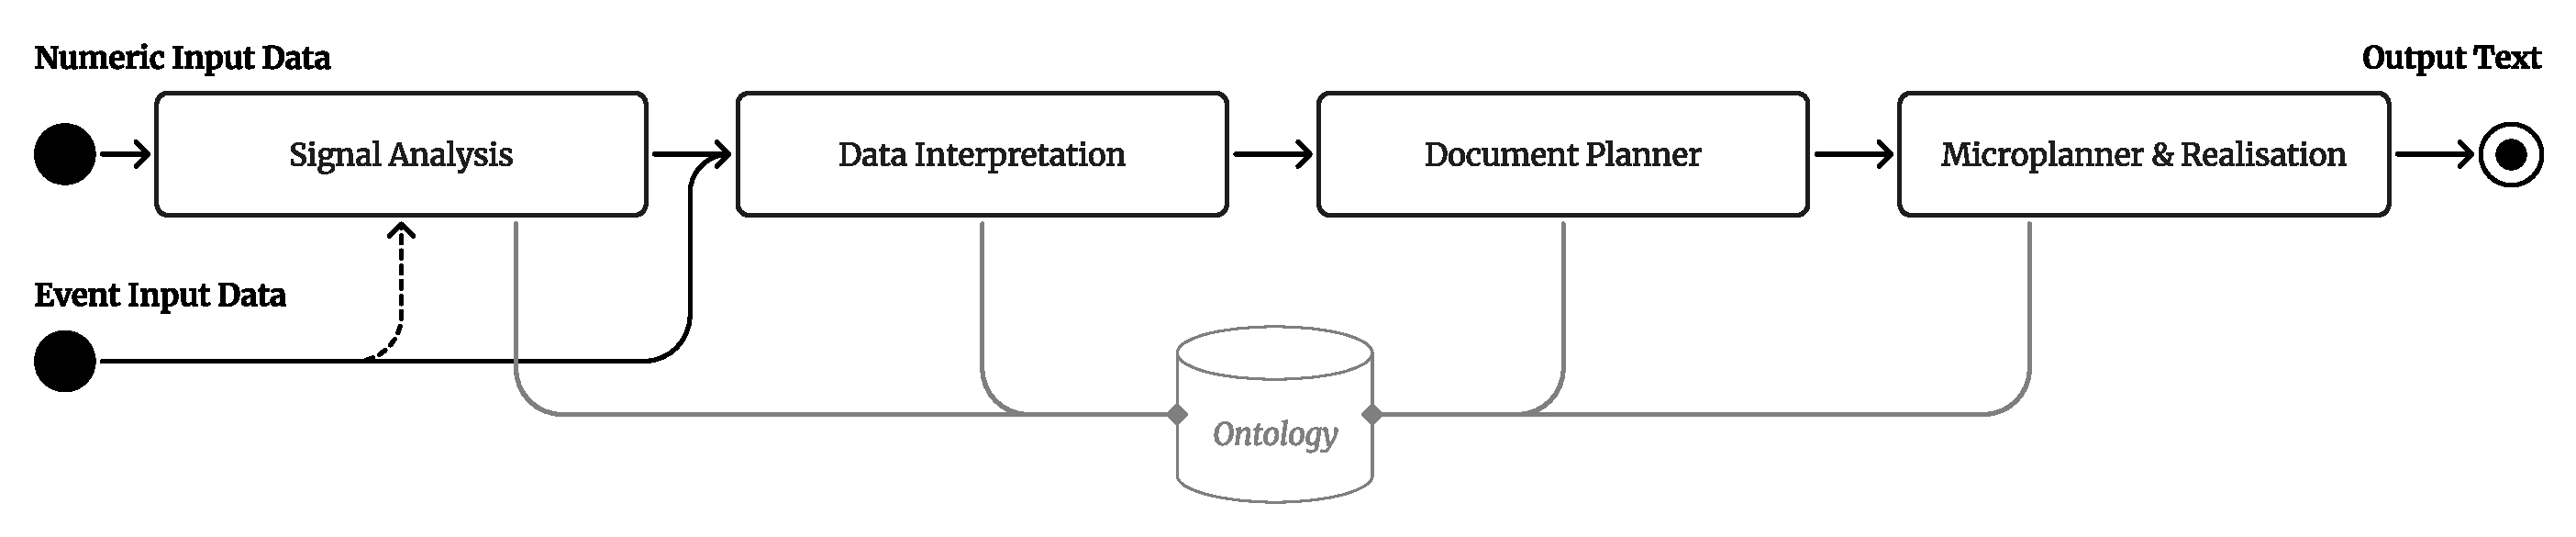
\includegraphics[width=\textwidth]{assets/pipeline-reiter.pdf}%
  }{%
    \fbox{\parbox{0.95\textwidth}{\centering Placeholder: missing file\\`assets/pipeline-reiter.pdf`}}%
  }
  \caption{The classic BabyTalk pipeline as proposed by \citet{reiter2007}. Continuous numeric data enters \textit{Signal Analysis}, while symbolic event data enters \textit{Data Interpretation}. Event data also supports Signal Analysis for pattern detection \cite{portet2008}.}
  \label{fig:pipeline-reiter}
\end{figure}

A critical challenge in D2T is bridging low-level data streams and high-level narrative events. Even statistical models often rely on intermediate structured representations \cite{chiang2025}; low-level data needs to be abstracted into reportable events via Signal Analysis \cite{portet2008}. Prior work spans rule-based detection, fuzzy logic \cite{ramos2019}, machine learning \cite{zhang2024}, and process mining \cite{zelst2021}. Within gaming, AlphaStar's StarCraft II work illustrates how rich game-state representations can capture complex dynamics \cite{mathieu2023}, even when summarization is not the primary goal.

\section{Sports and Game Commentary Generation}
Commentary generation for sports and games is a long-standing application of data-to-text systems, partly because outputs can often be checked against underlying data. We highlight work in both traditional sports and computer games that is relevant to esports commentary.

\subsection{Traditional Sports and Board Games}
Traditional sports and board games have provided benchmarks for post-game reporting and live commentary, supported by structured event logs and stable reporting conventions. This includes datasets like RotoWire \cite{wiseman2017} and reporting systems like PASS \cite{vanderlee2017}.

Work on live commentary spans early template systems such as ROCCO for RoboCup \cite{voelz1998} and neural models over event streams for soccer \cite{taniguchi2019}. Board-game commentary has also been explored in domains like chess \cite{zheng2025}, where the data volume differs substantially from esports.

Recent work increasingly uses LLMs downstream of event detection, for example from video \cite{andrews2024} or from match data \cite{cook2024}. Other systems emphasize retrieval or external knowledge for contextual depth (SCoReS \cite{lee2013}; Wikidata-enhanced PASS \cite{gatti2018}). These efforts motivate grounded realization, confirming that our setting must abstract higher-volume game-state data into reportable events.

\subsection{Esports Commentary}
Earlier game commentary work focused on \textit{Let's Play} content, informal first-person playthroughs targeting entertainment rather than competitive analysis, and reports substantial room for improvement in contextual relevance \cite{guzdial2018,shah2019,li2019}. Esports commentary is more demanding: it must convey strategic depth to a knowledgeable audience in real time. We review the most relevant work below.

Bardic \cite{barot2017} uses high-fidelity DotA2 data to generate world renders and text output, inferring player intentions by tracking actions over time windows and expressing them through hand-implemented story schemas.

\citet{elarewaju2020} used Probabilistic Lexicalized Tree-Adjoining Grammars (TAGs) trained on annotated caster data to generate text for esports highlights. The rule-based approach produced accurate event descriptions, though output quality was perceived as higher when paired with audiovisual content.

The work of \citet{wang2021} is closest to our setting, generating natural language commentary for League of Legends esports. They pair game-event data with commentary transcripts and train neural sequence models with hierarchical encoding, a technique that groups fine-grained game events into higher-level structures so they can be expressed as coherent sentences rather than fragmented lists. However, no viewer evaluation was reported in that work; \citet{wang2024} later conducted one at limited scale in follow-up research. A key limitation of the end-to-end framing is reduced control over content selection, which can cause misalignment between game events and generated text. \citet{wang2024} extend the approach with LLMs, finding Llama2-13B performs best on automatic metrics, but the core problem persists: the system still struggles to associate past game events with the current context, confirming that end-to-end framing alone is insufficient for coherent commentary. Together, these results motivate LLM-based realization paired with explicit upstream abstraction of game state.

\citet{zhang2022} compare rule-based and LLM-based realization for DotA2 event commentary, finding LLM realization outperforms rule-based on automated metrics, supporting the hybrid pipeline direction. \citet{zhang2024} take a different approach: rather than structured game data alone, they introduce GAME-MUG, a multimodal dataset for League of Legends commentary that combines game event logs, caster speech audio, and audience chat. They propose a joint multimodal dual learning model for game situation understanding and commentary generation. While our setting is text-only and structured-data-driven, their work highlights the potential of richer input modalities and audience-side signals for improving commentary quality.

\section{Summarization}
Selecting the most relevant events from a continuous stream and presenting them coherently is a challenge shared by live commentary generation and summarization alike. Reducing the amount of information for textual formats is something we have already mentioned for traditional sports as "OSC" \cite{lewandowski2012}. In esports, summarization and highlights are often regarded as the same, both identifying exciting moments, while true summarization also requires narrative coherence and explanatory context. Highlights can still provide a good baseline for narrative summarization, as they represent moments of the game worth highlighting.

\subsection{Highlight Detection}
Most existing work in esports highlight detection focuses on finding the ``best'' moments from audiovisual signals, rather than generating explanatory commentary. \citet{chu2017} reviewed computer-vision methods using visual features (e.g., motion intensity) and psycho-physiological proxies (e.g., chat/emotes). \citet{song2016} used Convolutional Neural Networks on visual features, and \citet{ringer2018} analyzed voice volume and facial expressions.

None of these methods use structured game data, relying instead on video and audio analysis. They identify exciting moments but do not explain why those moments matter, a gap that commentary generation can fill. We can learn from such systems by understanding if features like motion intensity are also captured in structured game data (e.g., unit production, battles).

\subsection{Narrative Summarization}
True summarization requires understanding causal links between events. The GameStory task \cite{lux2018, lux2019a, ninh2018, wutti2018} targeted this for CounterStrike, aiming to "boil down a long game to its most important events." Many submissions relied on heuristics (e.g., round start, bomb plant) and struggled to produce a cohesive story, showing that filtering alone is not enough for engaging, informative summaries.

To better use Large Language Models (LLMs) for reporting in games, \citet{kim2025} compress low-level game data into higher-level filtered representations to fit within a reduced context window. They evaluate analytical accuracy and identification of pivotal events, using heuristics (e.g., momentum changes based on win probabilities) to select important moments. This work is closely related, although summarization is treated primarily as a technical requirement for LLM use.

The gap lies in constructing narratives that go beyond event detection to explain the \textit{why} behind events.

\subsection{Event Relevance in Esports}
Selecting the right events is only part of the problem; summaries also require supportive information that explains \textit{why} an event matters in context. Research on supporting information in esports spectating shows that context matters: the right information must be shown at the right time \cite{charleer2018} (e.g., performance measures during a battle). However, little work directly addresses what is relevant for summaries in Age of Empires II (AoE2). Adjacent analyses, such as \citet{penney2021} on StarCraft II, identify described event types and supportive information. We will investigate these more in Chapter~\ref{chap:prelim} and Chapter~\ref{chap:viewer-study}.

\section{Evaluation of NLG Systems}
Evaluating the quality of generated text is a longstanding challenge in NLG. While standard automated metrics are widely used for benchmarking, they often fail to capture the nuances of narrative quality and reader engagement, which are central to this thesis.

\subsection{Automated Metrics}
The most common evaluation methods in NLG are n-gram overlap metrics such as BLEU \cite{papineni2002}, ROUGE \cite{lin2004}, and METEOR \cite{banerjee2005}. These metrics calculate a score based on the lexical similarity between the generated text and one or more human-written reference texts. While they are useful for tracking system improvements in tasks like machine translation, they have been shown to correlate poorly with human judgments of quality in open-ended generation tasks \cite{reiter2018,vanderlee2019,vanderlee2021}.

For creative domains like sports commentary, where there are many valid ways to describe the same event, these metrics are particularly limited. They cannot assess whether a narrative is exciting or insightful, only whether it uses the same words as the reference. Furthermore, they fail to measure factual correctness, a critical requirement for our system. As \citet{wang2021} noted in their work on esports commentary generation, standard metrics are unable to capture game-level strategic insights, which are essential for engaging commentary.

\subsection{Human Evaluation}
Given the limitations of automated metrics, human evaluation remains the gold standard for assessing NLG systems, but depends on the specific aims of the text \cite{vanderlee2019}. Human evaluation typically involves asking participants to rate generated texts on Likert scales. Automated metrics can be useful in constrained, reference-based tasks, but they struggle to assess \textit{Informativeness} (Does the text convey the necessary information?) and \textit{Enjoyment} (Is the text interesting and enjoyable to read?).

\noindent \Citet{vanderlee2019} emphasize the importance of using appropriate participant pools and clearly defined criteria to ensure reliability. In the context of esports, this means involving participants who are familiar with the game mechanics and terminology, as general readers may not be able to judge the accuracy or insightfulness of the commentary.

\subsection{Participant Recruitment for Esports Studies}
Recruiting participants familiar with the game is a real constraint when evaluating esports commentary systems. \citet{lux2019a} used professional game analyzers to verify summary quality; esports-related subreddits have also been shown to contribute substantial questionnaire respondents \cite{hamari2017} (In particular during the pandemic, when this research started.), with prior AoE2 questionnaires confirming this as an active channel for reaching the player and viewer community \cite{bidermayer2020}.

\subsection{Architectural Evaluation}
Beyond evaluating the final output, it is often necessary to assess the contribution of individual system components. \citet{callaway2002} proposed an architectural ablation approach for evaluating narrative generation systems. By systematically enabling and disabling specific modules (e.g., narrative planning, lexical choice), researchers can measure the impact of each component on the overall quality. This glass-box evaluation matters most for complex pipelines, where errors propagate from one stage to the next.

\section{Discussion and Gap Analysis}
The existing literature covers the components we need — modular pipelines, neural generation models, and linguistic work on what keeps audiences engaged — but a gap remains:
In the esports commentary systems we reviewed, many either rely on low-fidelity data (video pixels) or produce low-fidelity output (simple templates). Few have attempted to harness deep, structured game-state data (such as the data provided by CaptureAge) to generate high-level, strategic narratives.

Rule-based and hybrid data-to-text approaches can provide control over what is said and how it is expressed without requiring large amounts of annotated training data. We build on this by employing linguistic techniques and surfacing data that emphasizes information asymmetry between spectator and player.

Prior esports commentary systems primarily use event logs or metadata \cite{wang2021, wang2024, wang2025, barot2017, elarewaju2020, zhang2022} or multimodal broadcast cues \cite{zhang2024}; work using complete game-state data, like AlphaStar \cite{mathieu2023}, targets player AI rather than reporting. Across these directions, rigorous viewer-centered evaluation is rare, systems are often assessed via technical proxies rather than what viewers actually find useful, and it remains unclear how to turn high-fidelity game-state telemetry into efficient, state-aware strategic narratives grounded in esports communication research.

This thesis addresses these gaps in three concrete ways. First, we ground content selection and engagement strategies in a qualitative domain analysis of professional shoutcasting, informed by esports media studies (Chapter~\ref{chap:prelim}) and a preliminary viewer study (Chapter~\ref{chap:viewer-study}). Second, we use CaptureAge's high-fidelity game-state data to generate strategic narratives that go beyond what surface-level event logs or video can support (Chapter~\ref{chap:methods}). Third, we evaluate directly with the AoE2 viewer community using engagement-oriented measures derived from esports spectatorship research, rather than relying on automated proxy metrics (Chapter~\ref{chap:eval}).